\documentclass[10pt]{beamer}

\usetheme[progressbar=frametitle]{metropolis}
\usepackage{appendixnumberbeamer}
\usepackage{graphicx}

\usepackage{booktabs}
\usepackage[scale=2]{ccicons}

\usepackage{pgfplots}
\usepgfplotslibrary{dateplot}

\usepackage[utf8]{inputenc}
\usepackage[T1]{fontenc}
\usepackage{tikz}
\usetikzlibrary{matrix}

% \usepackage{blindtext}
% \usepackage{enumitem}
\usepackage{amsmath}

\usepackage{xspace}
\newcommand{\themename}{\textbf{\textsc{metropolis}}\xspace}

%% centralize
\newcommand{\vcenteredinclude}[1]{\begingroup
\setbox0=\hbox{\includegraphics{#1}}%
\parbox{\wd0}{\box0}\endgroup}

%% better: (general command to vertically center horizontal material)
\newcommand*{\vcenteredhbox}[1]{\begingroup
\setbox0=\hbox{#1}\parbox{\wd0}{\box0}\endgroup}

%% centralize

\title{Análise de tendências de resultados em ações financeiras}
% \subtitle{A modern beamer theme}
\date{\today}
\date{}
\author{Bernardo Flores Salmeron}
\institute{Universidade Federal da Bahia}
% \titlegraphic{\hfill\includegraphics[height=1.5cm]{logo.pdf}}

\begin{document}

\maketitle

% \begin{frame}{Table of contents}
%   \setbeamertemplate{section in toc}[sections numbered]
%   \tableofcontents[hideallsubsections]
% \end{frame}

\section{Introdução}

\begin{frame}[fragile]{Motivação}

  \begin{itemize}
  \item Ajuda na análise de dados para possíveis investidores
  \newline
  \item Análise do contexto histórico de valor de determinadas ações
  \newline
  \item Estudo do Método dos Mínimos Quadrados 
  \newline
  \end{itemize}

  % The \themename theme is a Beamer theme with minimal visual noise
  % inspired by the \href{https://github.com/hsrmbeamertheme/hsrmbeamertheme}{\textsc{hsrm} Beamer
  % Theme} by Benjamin Weiss.

  % Enable the theme by loading

  % \begin{verbatim}    \documentclass{beamer}
  %   \usetheme{metropolis}\end{verbatim}

  % Note, that you have to have Mozilla's \emph{Fira Sans} font and XeTeX
  % installed to enjoy this wonderful typography.
\end{frame}

\section{Método dos Mínimos Quadrados}
\begin{frame}[fragile]{Algoritmo para ajuste polinomial}
  \begin{itemize}
  \item Para uma equação com grau m a equação resultante será da forma  \begin{center}$f(x) = \beta_0 + \beta_1x^{1} + \beta_2x^{2} + \dots + \beta_mx^{m}$\newline\end{center}
  
  \item Para o ajuste polinomial de curvas, o sistema fica
igual a   
  \newline
  \[
    \begin{bmatrix}
      \sum{x_{i}^{0}} & \sum{x_{i}^{1}} & \sum{x_{i}^{2}} & \dots  & \sum{x_{i}^{m}} \\
      \sum{x_{i}^{1}} & \sum{x_{i}^{2}} & \sum{x_{i}^{3}} & \dots & \sum{x_{i}^{m+1}}\\
      \vdots & \vdots & \vdots & \ddots & \vdots \\
      \sum{x_{i}^{m}} & \sum{x_{i}^{m+1}} & \sum{x_{i}^{m+2}} & \dots  & \sum{x_{i}^{2m}} \\
    \end{bmatrix}
    .
    \begin{bmatrix}
      \beta_0 \\
      \beta_1 \\
      \vdots  \\
      \beta_m \\
    \end{bmatrix}
    =
    \begin{bmatrix}
      \sum{y_{i}} \\
      \sum{y_{i}x_{i}}\\
      \vdots \\
      \sum{y_{i}x_{i}^{m}} \\
    \end{bmatrix}
  \]
  \newline
  \end{itemize}
\end{frame}


\begin{frame}[fragile]{Algoritmo para ajuste polinomial}
  
  Por propriedade de matrizes na Álgebra 

  % \newline
  {\centering
    $A * X = B$\par
    $A^{-1} * A * X = A^{-1} * B$\par
    Por propriedade: $A^{-1} * A = I$\par
    $I * X = A^{-1} * B$\par
    Por propriedade: $I * X = X$\par
    $X = A^{-1} * B$\par
  }

\end{frame}

\begin{frame}[fragile]{Algoritmo para ajuste polinomial}
  
  Portanto, como $X = A^{-1} * B$
  \[
    \begin{bmatrix}
      \sum{x_{i}^{0}} & \sum{x_{i}^{1}} & \sum{x_{i}^{2}} & \dots  & \sum{x_{i}^{m}} \\
      \sum{x_{i}^{1}} & \sum{x_{i}^{2}} & \sum{x_{i}^{3}} & \dots & \sum{x_{i}^{m+1}}\\
      \vdots & \vdots & \vdots & \ddots & \vdots \\
      \sum{x_{i}^{m}} & \sum{x_{i}^{m+1}} & \sum{x_{i}^{m+2}} & \dots  & \sum{x_{i}^{2m}} \\
    \end{bmatrix}
    .
    \begin{bmatrix}
      \beta_0 \\
      \beta_1 \\
      \vdots  \\
      \beta_m \\
    \end{bmatrix}
    =
    \begin{bmatrix}
      \sum{y_{i}} \\
      \sum{y_{i}x_{i}}\\
      \vdots \\
      \sum{y_{i}x_{i}^{m}} \\
    \end{bmatrix}
    \implies
  \]

  \[
    \implies
    \begin{bmatrix}
      \beta_0 \\
      \beta_1 \\
      \vdots  \\
      \beta_m \\
    \end{bmatrix}
    =
    \begin{bmatrix}
      \sum{x_{i}^{0}} & \sum{x_{i}^{1}} & \sum{x_{i}^{2}} & \dots  & \sum{x_{i}^{m}} \\
      \sum{x_{i}^{1}} & \sum{x_{i}^{2}} & \sum{x_{i}^{3}} & \dots & \sum{x_{i}^{m+1}}\\
      \vdots & \vdots & \vdots & \ddots & \vdots \\
      \sum{x_{i}^{m}} & \sum{x_{i}^{m+1}} & \sum{x_{i}^{m+2}} & \dots  & \sum{x_{i}^{2m}} \\
    \end{bmatrix}^{-1}
    .
    \begin{bmatrix}
      \sum{y_{i}} \\
      \sum{y_{i}x_{i}}\\
      \vdots \\
      \sum{y_{i}x_{i}^{m}} \\
    \end{bmatrix}
  \]

\end{frame}

\begin{frame}[fragile]{Algoritmo para ajuste polinomial}
  
  Para esse trabalho foi implementado o ajuste polinomial para equações de primeiro e segundo grau

  Tendo os dados do gráfico deve-se então calcular a inversa da matriz A e a multiplicar pela matriz B para achar os coeficientes da função

  Foram utilizadas técnicas distintas para cálculo da matriz inversa para o ajuste para polinômios de grau um e dois  

  Portanto para achar a matriz de coeficientes deve-se aplicar duas operações:
  \begin{itemize}
    \item Achar o inverso de uma matriz
    \item Fazer multiplicações de matrizes
  \end{itemize}


\end{frame}


\begin{frame}[fragile]{Matriz inversa para ajuste de polinômio com grau um}
  
  Matriz da forma:                                   
  $\begin{bmatrix}
    \sum{x_{i}^{0}} & \sum{x_{i}^{1}} \\
    \sum{x_{i}^{1}} & \sum{x_{i}^{2}} \\
  \end{bmatrix} \newline $
  


  Para matrizes 2x2 a inversa pode ser calculada por
  \[
  \begin{bmatrix}
    {a} & {b} \\
    {c} & {d} \\
  \end{bmatrix}^{-1}
  = 
  \dfrac{1}{ad-bc}
  \begin{bmatrix}
    {d} & {-b} \\
    {-c} & {a} \\
  \end{bmatrix}
  \]

  No qual $ad-bc$ pode também ser representado como o determinante da matriz inicial

\end{frame}

\begin{frame}[fragile]{Matriz inversa para ajuste de polinômio com grau dois}
  
  Matriz da forma: 
  \[
  \begin{bmatrix}
    \sum{x_{i}^{0}} & \sum{x_{i}^{1}} & \sum{x_{i}^{2}} \\
    \sum{x_{i}^{1}} & \sum{x_{i}^{2}} & \sum{x_{i}^{3}} \\
    \sum{x_{i}^{2}} & \sum{x_{i}^{3}} & \sum{x_{i}^{4}}
  \end{bmatrix}
  \newline
  \newline
  \newline
  \newline\]



  

  A seguir serão mostrados os passos para o cálculo da inversa de uma matriz 3x3

\end{frame}

\begin{frame}[fragile]{Passos para o cálculo da inversa da matriz 3x3}
  
  Para uma matriz $A_{3x3}$:
  \begin{enumerate}
  \item Calcular o determinante da matriz A ($det(A))$
  
  \begin{center}
     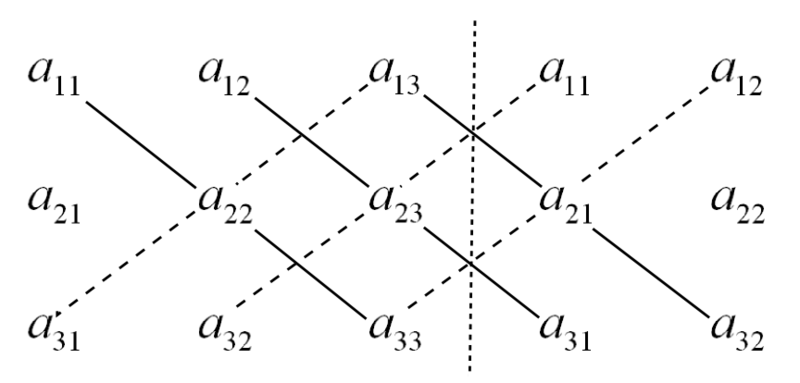
\includegraphics[scale=0.15]{images/determinante.png}  
  \end{center}
  
  \item Calcular a matriz de cofatores \newline
  Para uma posição (i, j):
    \begin{enumerate}
      \item Deve-se deletar os números presentes na mesma linha i e coluna j da matriz original e calcular a determinante dessa nova matriz 2x2
      \item Se i + j for múltiplo de dois o valor resultante é o próprio valor da determinante, caso contrário é o valor oposto da determinante
    \end{enumerate}
  Exemplo: 
    \[
    A = \begin{bmatrix}
      1 & 2 & 3 \\
      0 & 4 & 5 \\
      1 & 0 & 6
    \end{bmatrix}, 
    cfA_{11} = \begin{vmatrix}
      4 & 5 \\ 
      0 & 6 \notag
    \end{vmatrix}, 
    cfA_{12} = -\begin{vmatrix}
      0 & 5 \\ 
      1 & 6 \notag
    \end{vmatrix}
    =
    5    
    \]
  \end{enumerate}

\end{frame}

\begin{frame}[fragile]{Passos para o cálculo da inversa da matriz 3x3}
  \[
    cfA = \begin{bmatrix}
          24      &     5       & cfA_{13} \\
      cfA_{21} & cfA_{22} & cfA_{23} \\
      cfA_{31} & cfA_{32} & cfA_{33}
    \end{bmatrix}
  \]

  \begin{enumerate}
    \setcounter{enumi}{2}
    \item Transpor matriz de cofatores
    \[
      cfA = \begin{bmatrix}
        cfA_{11} & cfA_{12} & cfA_{13} \\
        cfA_{21} & cfA_{22} & cfA_{23} \\
        cfA_{31} & cfA_{32} & cfA_{33}
      \end{bmatrix},  
      \: tcfA = \begin{bmatrix}
        cfA_{11} & cfA_{21} & cfA_{31} \\
        cfA_{12} & cfA_{22} & cfA_{32} \\
        cfA_{13} & cfA_{23} & cfA_{33}
      \end{bmatrix}  
    \]
    \item Multiplicar toda os elementos da matriz transposta por $det(A)^{-1}$
    \[  
      inverse = \begin{bmatrix}
        tcfA_{11}*det(A)^{-1} & tcfA_{12}*det(A)^{-1} & tcfA_{13}*det(A)^{-1} \\
        tcfA_{21}*det(A)^{-1} & tcfA_{22}*det(A)^{-1} & tcfA_{23}*det(A)^{-1} \\
        tcfA_{31}*det(A)^{-1} & tcfA_{32}*det(A)^{-1} & tcfA_{33}*det(A)^{-1}
      \end{bmatrix}  
    \]
  \end{enumerate}

\end{frame}

\begin{frame}[fragile]{Multiplicação de Matrizes}

  O produto de matrizes A e B resultando na matriz C é obtido por meio da soma dos produtos dos elementos correspondentes da i-ésima linha de A pelos elementos da j-ésima coluna B.
  
  \[
  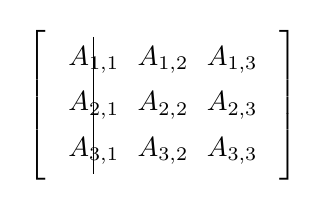
\begin{tikzpicture}
     \matrix (mat) [%
       matrix of nodes,
       left delimiter={[},right delimiter={]}
     ]
      {%
        $A_{1,1}$ & $A_{1,2}$ & $A_{1,3}$\\
        $A_{2,1}$ & $A_{2,2}$ & $A_{2,3}$\\
        $A_{3,1}$ & $A_{3,2}$ & $A_{3,3}$\\
        \\
      };
    % do the strike out thing
      % \draw[black] (mat-1-1.west)  -- (mat-1-3.east);
      \draw[black] (mat-1-1.north) -- (mat-3-1.south);
  \end{tikzpicture}
  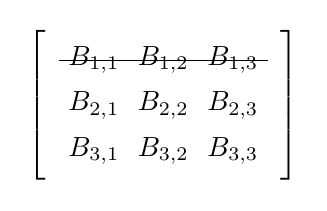
\begin{tikzpicture}

     \matrix (mat) [%
       matrix of nodes,
       left delimiter={[},right delimiter={]}
     ]
      {%
        $B_{1,1}$ & $B_{1,2}$ & $B_{1,3}$\\
        $B_{2,1}$ & $B_{2,2}$ & $B_{2,3}$\\
        $B_{3,1}$ & $B_{3,2}$ & $B_{3,3}$\\
        \\
      };
    % do the strike out thing
      \draw[black] (mat-1-1.west)  -- (mat-1-3.east);
      % \draw[black] (mat-1-1.north) -- (mat-3-1.south);
  \end{tikzpicture}
  \]
  \[
  =
  \]
  \[
  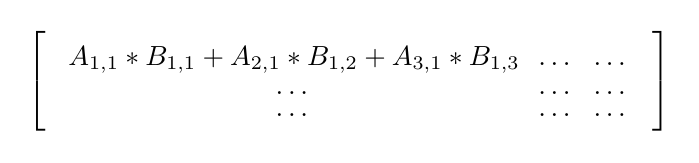
\begin{tikzpicture}
    \matrix (mat) [%
      matrix of nodes,
      left delimiter={[},right delimiter={]}
    ]
    {%
      $A_{1,1}*B_{1,1} + A_{2,1}*B_{1,2} + A_{3,1}*B_{1,3}$ & $\dots$ & $\dots$\\
      $\dots$ & $\dots$ & $\dots$\\
      $\dots$ & $\dots$ & $\dots$\\
      \\
    };
  \end{tikzpicture}

  \]

\end{frame}

\begin{frame}{Algoritmo para ajuste polinomial}

  Agora sabendo como fazer o calculo da matriz inversa e multiplicação de matrizes é só calcular a matriz $\beta$ de acordo com os dados obtidos
  \[
    \begin{bmatrix}
      \beta_0 \\
      \beta_1 \\
      \vdots  \\
      \beta_m \\
    \end{bmatrix}
    =
    \begin{bmatrix}
      \sum{x_{i}^{0}} & \sum{x_{i}^{1}} & \sum{x_{i}^{2}} & \dots  & \sum{x_{i}^{m}} \\
      \sum{x_{i}^{1}} & \sum{x_{i}^{2}} & \sum{x_{i}^{3}} & \dots & \sum{x_{i}^{m+1}}\\
      \vdots & \vdots & \vdots & \ddots & \vdots \\
      \sum{x_{i}^{m}} & \sum{x_{i}^{m+1}} & \sum{x_{i}^{m+2}} & \dots  & \sum{x_{i}^{2m}} \\
    \end{bmatrix}^{-1}
    .
    \begin{bmatrix}
      \sum{y_{i}} \\
      \sum{y_{i}x_{i}}\\
      \vdots \\
      \sum{y_{i}x_{i}^{m}} \\
    \end{bmatrix}
  \]
\end{frame}

\begin{frame}{Qualidade de ajuste}

    A qualidade de uma função ajustada u e pontos reais já obtidos representados por y é dada por
    \begin{center}
        $q = \sum_{i=1}^{N} (y_{i}-u_{i})$
    \end{center}
    em que $N$, consiste no número de pontos
    
    Observe que quanto menor for o valor $q$ mais precisa é a função
\end{frame}

\section{Análise de Ação}

\begin{frame}{Obtenção dos dados}

  Para esse trabalho foi utilizado dados da empresa Facebook, Inc. (ação FB) durante o período de 
  \begin{itemize}
    \item 13/05/2013 até 24/09/2018
    \item 02/04/2018 até 09/11/2018
  \end{itemize}
  
  \begin{center}
    
\includegraphics[scale=0.10]{images/facebook.png}
  \end{center}
  Os dados podem ser baixados através do site Yahoo finanças \newline
  Link: \url{https://finance.yahoo.com/quote/FB?p=FB}
\end{frame}

\begin{frame}{Aplicação do Algoritmo}

  Após a obtenção dos dados da ação FB os seguintes procedimentos foram feitos para cada período:
  \begin{itemize}
      \item Ajustes linear e quadrático 
      \item Plotagem de gráfico para cada ajuste 
      \item Análise de qualidade de cada ajuste 
      \item Comparativo de diferentes ajustes para um mesmo período 
  \end{itemize}
\end{frame}

\begin{frame}{Período de 13/05/2013 até 24/09/2018}

  Dados reais do Período
  
  \includegraphics[scale=0.6]{"images/fbl-real".png}
\end{frame}

\begin{frame}{Período de 13/05/2013 até 24/09/2018 - Ajuste Linear}

  Equação da reta após ajuste para uma equação linear:
  \begin{center}
  $u = f(x) = 0.545256449x + 32.3944553676$
  
  $q = \sum_{i=1}^{N} (y_{i}-u_{i}) = 35464.9446729667$
  \end{center}
  
  \begin{center}
    \includegraphics[scale=0.45]{"images/fbl-linear".png}
  \end{center}
\end{frame}

\begin{frame}{Período de 13/05/2013 até 24/09/2018 - Ajuste Quadrático}

  Equação da reta após ajuste para uma equação quadrático:
  \begin{center}
  $u = f(x) = -0.0000545252x^2 + 0.5609597066x + 31.6433162106$
  
  $q = \sum_{i=1}^{N} (y_{i}-u_{i}) = 35499.0004518346$
  \end{center}
  
  \begin{center}
    \includegraphics[scale=0.45]{"images/fbl-quadratico".png}
  \end{center}
\end{frame}

\begin{frame}{Período de 13/05/2013 até 24/09/2018 - Comparativo}

  Comparativo entre dados reais, ajuste linear e ajuste quadrático
  
  \begin{center}
    \includegraphics[scale=0.6]{"images/fbl-both".png}
  \end{center}
\end{frame}

\begin{frame}{Período de 02/04/2018 até 09/11/2018}

  Dados reais do Período
  
  \begin{center}
    \includegraphics[scale=0.6]{"images/fbreal".png}
  \end{center}
\end{frame}


\begin{frame}{Período de 02/04/2018 até 09/11/2018 - Ajuste Linear}

  Equação da reta após ajuste para uma equação linear:
  \begin{center}
  $u = f(x) = -0.1849197185x + 189.5355026317$
  
  $q = \sum_{i=1}^{N} (y_{i}-u_{i}) = 41251.7195782369$
  \end{center}
  
  \begin{center}
    \includegraphics[scale=0.45]{"images/fblinear".png}
  \end{center}
\end{frame}

\begin{frame}{Período de 02/04/2018 até 09/11/2018 - Ajuste Quadrático}

  Equação da reta após ajuste para uma equação quadrática:
  \begin{center}
  $u = f(x) = -0.0069320225x^2 + 0.9242038877x + 160.1437270675$
  
  $q = \sum_{i=1}^{N} (y_{i}-u_{i}) = 12439.3368638241$
  \end{center}
  
  \begin{center}
    \includegraphics[scale=0.45]{"images/fbquadratico".png}
  \end{center}
\end{frame}


\begin{frame}{Período de 02/04/2018 até 09/11/2018 - Comparativo}

  Comparativo entre dados reais, ajuste linear e ajuste quadrático
  
  \begin{center}
    \includegraphics[scale=0.6]{"images/fbboth".png}
  \end{center}
\end{frame}

\end{document}
